% !TeX spellcheck = hu_HU
\documentclass[12pt,a4paper]{article}
\usepackage[utf8]{inputenc}
\usepackage{cmap}
\usepackage[T1]{fontenc}
\usepackage[magyar]{babel}
\usepackage{amsmath}
\usepackage{amsfonts}
\usepackage{amssymb}
\usepackage{graphicx}

\usepackage{outlines}
\usepackage{hyperref}

\hyphenpenalty=10000

\begin{document}

\begin{center}
	\huge
	Formális nyelvek és fordítóprogramok alapjai\\
	\vspace{1mm}
	\LARGE
	Fordítóprogramok témakör jegyzete\\
	\vspace{5mm}
	\large
	Készült Dévai Gergely előadásai és gyakorlatai alapján\\
	\vspace{5mm}
	Sárközi Gergő, 2021-22-2. félév\\
	Nincsen lektorálva!
\end{center}

\tableofcontents

\pagebreak

\section{Fordítóprogramok bevezetés}

\begin{outline}
	\1 Fordítóprogram lényege: magas szintű és gépi kód között áthidal
	\1 Fordítás (compiler) vs értelmezés (interpreter)
		\2 Fordítás: optimalizálás, alaposabb ellenőrzés, platformonként
		\2 Értelmezés: rugalmasabb, csak futási idő van (pl. Python)\\
		Dinamikus bemenet is futtatható egyszerűen
	\1 Virtuális gép (JVM, CLR): fordított kód (bájtkód, CLI) értelmezése
	\1 JIT: bájtkód fordítása gépi kódra futási időben (cél: gyorsítás)
		\2 Kezdetben csak értelmezés, hot spots-ok keresése
		\2 Ezután hot spots-ok lefordítása gépi kódra
			\3 Extra: futási idejű infókat is fel lehet használni fordításkor
		\2 Miért nem mindent induláskor? $\implies$ lassú indulás
\end{outline}

\subsection{Fordítás és szerkesztés}

\begin{outline}
	\1 Statikus könyvtár (.a, .lib):
		\2 Beépül a futtatható állományba
	\1 Dinamikus könyvtár (.so, .dll):
		\2 Pozíciófüggetlen objektumok vannak benne
		\2 Függőség, hivatkozás egy rendszeren jelen levő könyvtárra
		\2 Ugyan azt a példányt használja minden processz
		\2 Csak programkódról van szó, nincs közös memória
\end{outline}

\pagebreak

\subsection{Fordítóprogramok logikai felépítése}

\begin{outline}
	\1 Bemenet: forráskód
	\1 Analízis: lexikális, szintaktikus, szemantikus elemzés (ez a sorrend)
		\2 Minden hibának ki kell itt derülnie
		\2 Lexikális elemzés:
			\3 Kimenet: tokenek (lexikális elemek) sorozata
			\3 Whitespace-t általában figyelmen kívül hagyjuk
		\2 Szintaktikus elemzés:
			\3 Kimenet: szintaxisfa
			\3 Tokenek belső szerkezetének feltérképezése, ellenőrzése
			\3 Token: szintaktikus elemzés nyelvtanának terminális szimbóluma
		\2 Szemantikus elemzés: (statikus szemantika)
			\3 Kimenet: szintaxisfa attribútumokkal, szimbólumtábla
				\4 Attribútum példa: milyen típusú egy kifejezés
				\4 Szimbólumtábla példa: milyen típusú egy változó
			\3 pl. változó deklarálva volt-e, típushelyes-e minden
	\1 Szintézis: kódgenerálás, optimalizálás
		\2 Általában nem egy lépés, hanem transzformációk sorozata
		\2 Váltják egymást, először valami köztes nyelv, végül tárgykód
		\2 Kódgenerálás:
			\3 Nem érdemes egyből gépi kódra fordítani
			\3 magas szint $\to$ (fordító) $\to$ Assembly $\to$ (assembler) $\to$ gépikód
		\2 Optimalizálás:
			\3 Példa: szintaxisfa optimalizálás $\to$ kódgen. $\to$ assembly optim.
	\1 Kimenet: tárgykód
\end{outline}

\pagebreak

\section{Lexikális elemzés (scanner / lexer)}

\subsection{Bevezetés}

\begin{outline}
	\1 Feladat: forrásszöveg elemi egységekre bontása
	\1 Bemenet: karaktersorozat
	\1 Kimenet: lexikális elemek (tokenek)
	\1 Eszközök: reguláris kifejezések, véges determinisztikus automaták
\end{outline}

\subsection{Whitespace, kommentek}

\begin{outline}
	\1 Whitespace fel van ismerve, de nem készül belőle token
	\1 Behúzás-érzékeny nyelvek: számon van tartva, készül belőle behúzás szintet növelő/csökkentő token
	\1 Kommenteket is felismeri a lexer, ebből sem készül token
\end{outline}

\subsection{Tokenizálás}

\begin{outline}
	\1 Egy tokenhez a reguláris kifejezés általában elég egyszerű, hiszen ezek az elemi (legkisebb) egységek.
	\1 A leghosszabb illeszkedést keressük: addig vesszük a következő karaktert, amíg már semmi nem illeszkedik. Ekkor az előző karaktersorozatra illeszkedő regexek közül vesszük a sorrendben az elsőt.
		\2 Leghosszabb illeszkedés elve: leghosszabb illeszkedést keressük
		\2 Prioritás elve: több regex közül a sorrendben az első "nyer"
		\2 A leghosszabb illeszkedés fontosabb, mint a sorrend
	\1 Implementáció:
		\2 Reguláris kifejezést VDA-vá alakítjuk
		\2 VDA implementáció: elágazásokkal / táblázattal
\end{outline}

\pagebreak

\subsubsection{Tokenekhez csatolt információk}

\begin{outline}
	\1 Minden tokenhez: pozíció (első és utolsó karakter: sor és oszlopszám)
		\2 Hibaüzenetekhez szükséges
	\1 Azonosítókhoz, literálokhoz: a megadott érték (lásd szemantikus elemzés)
\end{outline}

\subsubsection{Lexikális hibák}

\begin{outline}
	\1 Akkor van hiba, ha semmi nem match-elt
	\1 Egyszerű megoldás: egy karaktert kidobunk (kiírunk hibát), többi karakterrel folytatjuk az elemzést
	\1 Példa: illegális karakter (karakter nincs a nyelv abécéjében)
	\1 Példa: lezáratlan string (hiba a sor végén derül ki)
	\1 Példa: lezáratlan többsoros megjegyzés (fájl végén derül ki)
\end{outline}

\pagebreak

\section{Szintaktikus elemzés (syntax checker)}

\subsection{Bevezetés}

\begin{outline}
	\1 Feladat: forrásszöveg szerkezetének felderítése, formai ellenőrzése
	\1 Bemenet: tokenek
	\1 Kimenet: szintaxisfa és szintaktikus hibák
	\1 Eszközök: környezetfüggetlen nyelvtanok, veremautomaták
\end{outline}

\subsection{Szintaxisfa}

\begin{outline}
	\1 Levelek balról jobbról olvasva kiadják a bemeneti tokeneket
	\1 Grammatika alapján jön létre; az szabályozza, hogy mi megengedett
\end{outline}

\subsection{Nyelvtan elvárt tulajdonságai}

\begin{outline}
	\1 Redukáltság: nincsenek felesleges nemterminálisok
	\1 Ciklusmentesség: az baj, ha $A$-ból eljuthatunk $A$-ba anélkül, hogy bármilyen terminálist előállítanánk
	\1 Egyértelműség: minden szóhoz pontosan egy szintaxisfának kell tartoznia
		\2 Többféle levezetés szabályos, ez mást jelent!
\end{outline}

\subsection{Nem egyértelmű szintaxisfa megoldása}

\begin{outline}
	\1 Példa: nyelvtan számok összeadására (Bonyolítás: szorzást is belevesszük)
		\2 Helytelen: $E \to \mathbb{N} \;|\; E + E$
		\2 Helyes: $E \to \mathbb{N} \;|\; E + \mathbb{N}$
	\1 Operátor precedencia megadása (erre a példa nem tér ki)
	\1 Operátor asszociativitásának megadása
\end{outline}

\subsection{Szintaxisfa felépítése}

\begin{outline}
	\1 Két fő család: felülről lefelé és alulról felfelé
\end{outline}

\pagebreak

\subsubsection{Felülről lefelé elemzés (pl. ANTLR)}

\begin{outline}
	\1 Startszimbólumból indulva terminálisok felé haladunk
	\1 Input feldolgozása: balról jobbra
	\1 Legbaloldalibb levezetés: több terminális esetén a legbaloldalibb
	\1 Előreolvasás: következő pár token alapján válasszunk szabályt
		\2 Egy nyelvtan LL(k) tulajdonságú, ha felülről lefelé elemzés során legfeljebb $k$ token előreolvasásával meghatározható a legbaloldalibb feldolgozatlan nemterminálishoz alkalmazandó nyelvtani szabály
		\2 Van olyan nyelvtan, amihez nem létezik ilyen $k$, de a programozási nyelvek nyelvtanai nem ilyenek
	\1 Legyen $\alpha$ egy tetszőleges szimbólumsorozat: terminálisok és nemterminálisok
	\1 $FIRST_1(\alpha) = \alpha$-ból levezethető szimbólumsorozatok első karakterei
		\2 $\epsilon$ része ha az üres szó levezethető, továbbá $FIRST_1(\epsilon) = \{\epsilon\}$
		\2 $\alpha$ egy terminálissal kezdődik $\implies$ az a terminális az eredmény
	\1 $FOLLOW_1(\alpha)=$ kezdőszimbólumból levezethető szimbólumsorozatokban milyen terminálisok állhatnak $\alpha$ után
		\2 $\alpha$ a levezethető szimbólumsorozat legvége $\implies$ \# kerül a halmazba
		\2 Kiszámolása nem triviális a rekurzív szabályok miatt
	\1 Rekurzív leszállás: LL(1) elemzés egy implementációja
		\2 LL: Left to right, using Leftmost derivation
		\2 Legyen minden nemterminális egy függvény és minden szabályalternatíva egy-egy elágazás-ág (hibakezelés külön ágban)
		\2 Szabály jobboldal: terminálishoz $accept$, nemterminálishoz fv hívás
			\3 $accept$: tovább olvasás ha next == paraméter, egyébként hiba
		\2 Elágazás feltételek megírása, kiszámolása:
			\3 Legyen a szóban forgó szabály: $A \to \alpha$
			\3 $FIRST_1(\alpha)$ halmaz kiszámolása, ha van benne $\epsilon$, akkor kivesszük és vesszük az uniót a $FOLLOW_1(A)$ halmazzal
			\3 Ezen elemek a feltételek: $next == x_1 \;||\; next == x_2 \;||\; ...$
		\2 Tétel: környezetfüggetlen nyelvtan pontosan akkor LL(1) tulajdonságú, ha bármely $A \to \alpha$, $A \to \beta$ szabályokra a fenti feltételek diszjunktak
		\2 Van verem: a call stack
		\2 Név eredete: rekurzív nyelvtan esetén rekurzív függvény hívások
\end{outline}

\begin{figure}[h!]
	\centering
	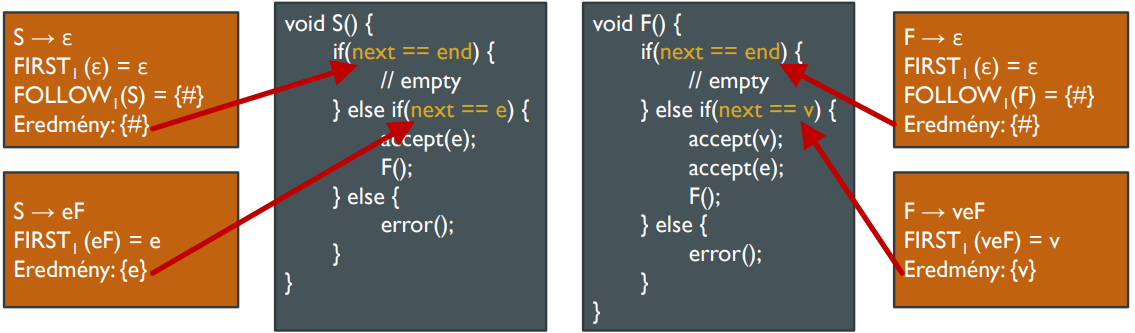
\includegraphics[width=1\linewidth]{LL1}
\end{figure}

\begin{outline}
	\1 Ábra: felülről lefelé elemzés, LL(1), rekurzív leszállás
\end{outline}

\subsubsection{Alulról felfelé elemzés (pl. Bison)}

\begin{outline}
	\1 Terminálisokból indulva a startszimbólum felé építjük a fát
	\1 Input feldolgozása: balról jobbra
	\1 Legjobboldali levezetés inverzét állítja elő
	\1 Van olyan nyelvtan, amit ez támogat de a felülről lefelé elemzés nem
	\1 LR(1) elemzés: Left to right, using Rightmost derivation
	\1 Léptetés: következő token elhelyezése verem tetején
	\1 Redukció: veremben lévő szabály jobboldal helyettesítése szabály baloldallal, közben a 	szintaxisfa bővítése
		\2 Nem feltétlenül csökkenti a verem méretét: $\epsilon$ szabály 1-gyel növeli
	\1 Egy nyelvtan LR(k) tulajdonságú, ha legfeljebb $k$ token előreolvasásával meghatározható, hogy léptetés vagy redukció jöjjön és redukció esetén a használandó szabály is kiderül
	\1 LR(1) elemzés implementálása; léptetés vagy redukció eldöntése
		\2 Előreolvasás és pillanatnyi állapot alapján (tehát táblázat)
		\2 Verem: tokeneket és állapotokat tárol (nem hagyományos VDA)
		\2 Kezdő állapot: 0 (nincs hozzárendelt bemenet, csak állapot van)
		\2 Bemenet lehet: terminális, nemterminális (kivéve $S$), input vége
		\2 Elfogadás: $S \to ...$ szabály és input vége "találkozása" esetén
		\2 Táblázat létrehozása nyelvtanból: nem a tananyag része
		\2 Tétel: környezetfüggetlen nyelvtan pontosan akkor LR(1) tulajdonságú, ha a táblázat konfliktusmentesen kitölthető
\end{outline}

\begin{figure}[h!]
	\centering
	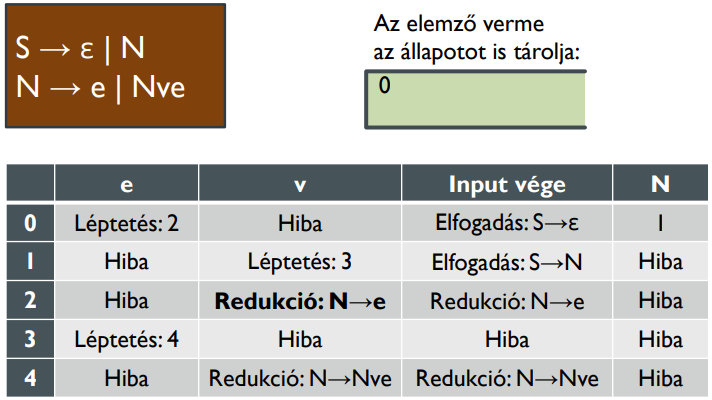
\includegraphics[width=0.7\linewidth]{LR1}
\end{figure}

\begin{outline}
	\1 Ábra: Alulról felfelé elemzés, LR(1)
	\2 Oszlopok: bemenet vagy nemterminális
	\2 Sorok: pillanatnyi állapot
	\2 Cellák: mit kell tenni és hogyan (nemterminális esetén csak állapot)
		\3 Léptetés: verembe helyezni a bemenetet és az odaírt számot
		\3 Redukció: veremben szabály jobboldal helyettesítése baloldallal
			\4 Új "bemenet": a nemterminális (a szabály baloldal)
			\4 Új állapot: baloldali nemterminális oszlopából a szám,
			de előbb pop-olni kell a vermet: ott maradt állapot sora kell
		\3 Elfogadás: speciális redukció: készen vagyunk
\end{outline}

\subsubsection{Backtracking (extra, nem az anyag része)}

\begin{outline}
	\1 Lassú és nem tudjuk meg, hogy hol a hiba: annyit kapunk vissza, hogy sehogy sem sikerült illeszteni a bemenetet
	\1 Ezen okokból nem használjuk fordítóprogramokra; vannak jobb megoldások
\end{outline}

\pagebreak

\section{Szemantikus elemzés (semantic analyzer)}

\subsection{Bevezetés}

\begin{outline}
	\1 Feladat: statikus szemantika (pl. változó deklaráltsága, típusa) ellenőrzése
	\1 Bemenet: szintaxisfa
	\1 Kimenet: szintaxisfa attribútumokkal, szimbólumtábla (+hibák)
	\1 Eszközök: attribútumnyelvtanok
\end{outline}

\subsection{Feladatok kategóriái}

\begin{outline}
	\1 Szimbólumtábla
		\2 Deklarációk feldolgozása
		\2 Azonosítószimbólumok deklarációhoz kötése
		\2 Hatókör, láthatóság szabályok ellenőrzése
			\3 Hatókör: hol létezik
			\3 Láthatóság: hol érhető el
	\1 Attribútumnyelvtan
		\2 Típusellenőrzés, típuslevezetés
		\2 Típuskonverziók
	\1 Warning-ok (pl. konstans nullával osztás)
		\2 Ezzel mi nem foglalkozunk
\end{outline}

\pagebreak

\subsection{Szimbólumtábla}

\begin{outline}
	\1 Oszlopai:
		\2 Név: szöveg
		\2 Fajta: függvény, paraméter, lokális változó, stb.
		\2 Típus: $int \to void$, $int$, stb.
		\2 Deklaráció: pl. 1. sor, 10. oszlop
		\2 Használat: pl. 3. sor,  10. oszlop, ... (lista)
	\1 Beszúrás: új deklaráció esetén
		\2 Beszúrás előtt mindig keresés van: újradeklarálás tiltása
	\1 Keresés: szimbólum neve alapján kereshetünk
		\2 Használatát érdemes feljegyezni (pl. refaktorálás miatt)
	\1 Implementáció veremként:
		\2 Beszúrás: tetejére ($push$)
		\2 Keresés: fentről (tetejéről) lefelé, első találatnál megállunk
	\1 Blokk-index vektor (ez is egy verem)
		\2 Új blokk esetén elmentjük a szimbólumtábla-verem tetejét ($push$)
		\2 Blokkból kilépés esetén:
			\3 Törlés tábla-veremből ($pop$), amíg teteje nem a mentett érték
			\3 Lementett értéket kitöröljük a blokk-index vektorból ($pop$)
	\1 Újradeklarálás megtiltása, de egyes elfedések megengedése
		\2 Újradeklarálás miatti kereséskor nem megyünk végig a szimbólumtáblán
		\2 Blokk-index teteje által mutattot deklaráció felett (exkluzív) keresünk
		\2 Üres a blokk-index vektor $\implies$ egész szimbólumtáblában keresünk
\end{outline}

\pagebreak

\subsection{Típusrendszerek}

\begin{outline}
	\1 Statikus (fordítási időben történik a típusellenőrzés)
		\2 Futás időben nem kell típusinformációt tárolni
			\3 Kivétel: Java instanceof, C++ alosztályok
		\2 Sikeres fordítás esetén nem lehet futási idejű típushiba
			\3 Kivétel: fordítás és futás idejű könyvtár verziók eltérnek
		\2 pl. Ada, C++, Haskell
	\1 Dinamikus (futási időben történik a típusellenőrzés)
		\2 Futási időben típusokat is kell tárolni, nem csak értékeket
		\2 Utasítások végrehajtása előtt típushelyességet ellenőrizni kell
		\2 Futási időben derülnek ki egyes hibák, cserébe flexibilisebb
		\2 pl. Lisp, Erlang
\end{outline}

\subsection{Ki adja meg a típusokat?}

\begin{outline}
	\1 Programozó adja meg: deklarációk típusozottak
		\2 Több lehetőség típusellenőrzésre
		\2 Egyszerűbb fordítóprogram, gyorsabb fordítás
	\1 Típuskikövetkeztetés, típuslevezetés: deklarációk általában típus nélkül
		\2 Műveletek alapján fordítóprogram kitalálja a kifejezés típusát
		\2 Kényelmes programozni, de olvashatóságért érdemes típusozni
		\2 pl. Haskell
\end{outline}

\subsection{Típuskonverzió}

\begin{outline}
	\1 Egy kifejezés típusát változtatja meg
	\1 Lehet automatikus (implicit) vagy manuális (explicit)
	\1 Osztályhierarchia miatti típuskonverzió is van (szülő osztály metódusa)
	\1 Típuskonverzió miatt az érték is megváltozhat (pl. int-ből double)
\end{outline}

\pagebreak

\subsection{Attribútumnyelvtan}

\begin{outline}
	\1 Szintaxist leíró nyelvtan szimbólumaihoz attribútumokat rendelünk
		\2 Szemantikus elemzéshez kell (deklaráltság-, típusellenőrzés)
		\2 Kódgeneráláshoz kell (literál értéke, maga a kód)
		\2 Kódoptimalizáció számára is kell
	\1 Szabályokhoz akciókat (programkódot) rendelünk
		\2 Szemantikus ellenőrzést végzünk
		\2 Kiszámoljuk pl. a szabály baloldal típusát a jobboldal típusaiból
		\2 Azonosító esetén a szimbólumtáblát használjuk:
			\3 Neve alapján lekérdezzük a szimbólumtáblát
			\3 Megnézzük, hogy deklarált-e és mi a típusa
		\2 Szimbólum többször szerepel szabályban: sorszámozzunk
	\1 Szintetizált attribútum:
		\2 Szabály bal oldalán állt, amikor kiszámoltuk (bal oldal kap értéket)
		\2 Alulról felfelé közvetít információt a szintaxisfában
		\2 pl. kifejezés típusa
	\1 Kitüntetett szintetizált attribútum: lexikális elemző ad neki értéket
		\2 Ehhez módosítani kell a lexikális elemzőt (ne csak tokent adjon)
		\2 pl. azonosító neve, literál értéke
	\1 Örökölt attribútum (ciklus példával szemléltetve)
		\2 Start szabályoknál ($S \to ...$) hamisra állítani a jobb oldalt
		\2 Normális szabályoknál a bal oldal értékét örökli a jobb oldal
		\2 Ciklus szabály: igazra állítjuk a jobb oldal megfelelő szimbólumát
		\2 Fentről lefelé terjed az információ a szintaxisfában
		\2 Bisonban ilyen nincsen
			\3 Ezt S-attribútumnyelvtannak hívjuk (nincsenek örökölt attribútumok)
			\3 Örökölt attribútumok nem illeszkednek jól az LR elemzéshez
			\3 Megoldás: szimbólumtábla használata ilyenkor (nem tananyag)
	\1 Megszorítások, elvek, szabályok
		\2 Csak az adott szabály bal és jobb oldalával foglalkozunk
			\3 Nem olvasunk a fán feljebb vagy lejjebb
			\3 Ha szükséges, akkor definiálunk szabályokat és segítségükkel egyesével hordozunk információt a szintaxisfa szintjein
		\2 Egy attribútumértéket csak egy akció határozhat meg
			\3 Ha több akció is ugyan azt az értéket írja felül, az baj
	\1 Nem triviális, hogy az akciókat milyen sorrendben futtatjuk
		\2 Indoklás: ha ez egyik akció felhasználja egy másik akció eredményét...
	\1 Attribútumok és kód generálás összefüggése
		\2 Generált kód is lehet egy attribútum
		\2 Kódgenerálásnál gondolni kell az attribútumok kiszámítási sorrendjére
\end{outline}

\pagebreak

\section{Assembly}

\subsection{Bevezetés}

\begin{outline}
	\1 Assembly: alacsony szintű, hardverközeli programozási nyelvek csoportja
	\1 Assembler: fordítóprogram assembly-ről gépi kódra
	\1 Mi 32 bites, x86-os architektúrát, NASM szintaxisú assembly-t használunk
\end{outline}

\subsubsection{C használat (\texttt{extern} függvények)}

\begin{outline}
	\1 Pár függvény C-ben (\texttt{io.c}) van megírva egyszerűség kedvéért
		\2 Assembly-ben túl sok időbe tellene megcsinálni
	\1 Függvények: \texttt{write\_natural}, \texttt{read\_natural},
	\texttt{write\_boolean}, \texttt{read\_boolean}
\end{outline}

\subsubsection{Fordítás}

\begin{outline}
	\1 \begin{verbatim}nasm -felf Xyz.asm && gcc -m32 io.c Xyz.o -o Xyz\end{verbatim}
	\1 Xyz-t ki kell cserélni valami értelmes névre
	\1 \texttt{-m32}: 32 bites mód (64 bites OS esetén is)
\end{outline}

\subsection{Általános információk}

\begin{outline}
	\1 Komment: ; után
	\1 Méretek: byte (1), word (2), dword (4)
	\1 abc|xyz jelentése: két memória/regiszter terület egymás után olvasandó
		\2 Szám esetén a magasabb helyi érték van bal oldalt (intuitív)
\end{outline}

\pagebreak

\subsection{Adattárolás}

\subsubsection{Regiszterek}

\begin{outline}
	\1 Gyors, kis kapacitás, pillanatnyi művelet operandusai itt vannak általában
	\1 Általános célú regiszterek: eax, ebx, ecx, edx, esi, edi
	\1 Speciális regiszterek:
		\2 eip: instruction pointer, következő végrehajtandó utasításra mutat
		\2 eflags: jelző bitek (pl. aritmetikai művelet során van beállítva)
	\1 C-ből hívott függvényben csak ezeket szabad módosítani: eax, ecx, edx
		\2 A tárgyban nekünk az összes kódunk ilyen
		\2 Ha mégis módosítjuk, vissza kell őket állítani
		\2 Összes regiszter mentése/visszaállítása: \texttt{pusha}, \texttt{popa}
\end{outline}

\begin{figure}[h!]
	\centering
	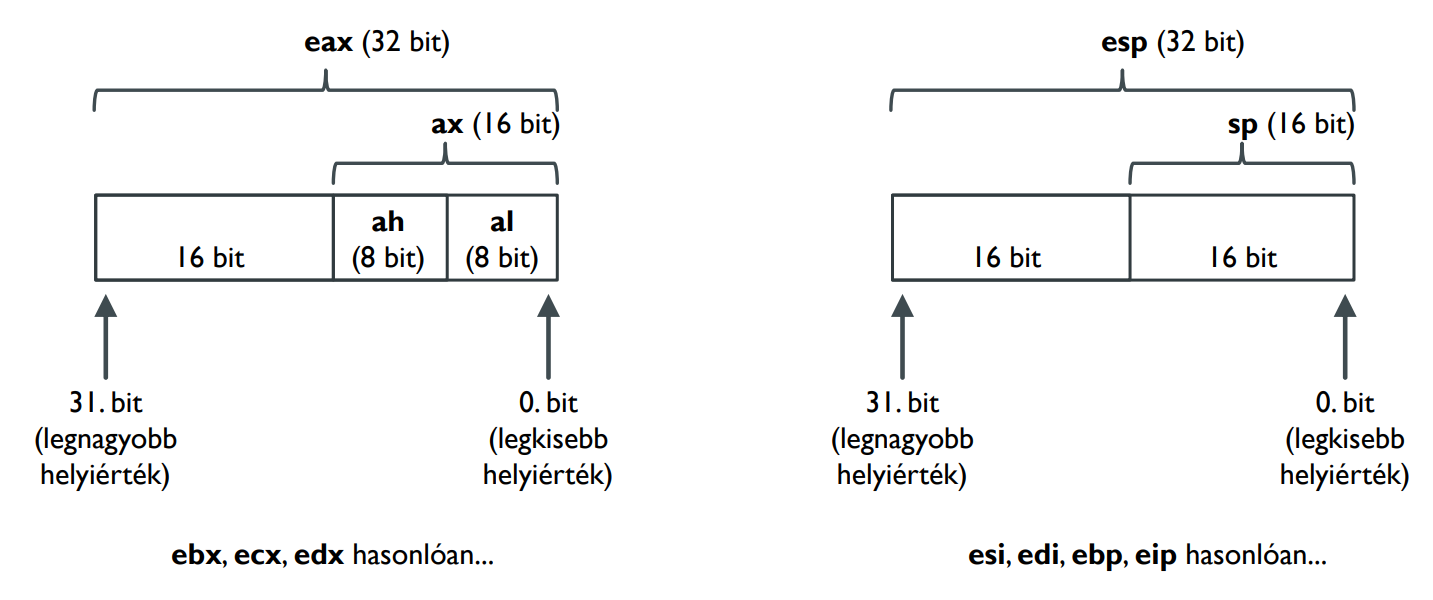
\includegraphics[width=0.65\linewidth]{regiszterek-szerkezete}
\end{figure}

\subsubsection{Verem}

\begin{outline}
	\1 Itt van: fv paraméter, fv visszatérési érték, fv lokális változó (!!!)
	\1 0 felé nő, ezért így is lehet törölni (pop) belőle:\texttt{add esp,N}
	\1 esp: stack pointer, verem tetejére mutat
		\2 Verembe push után csökken az értéke
	\1 ebp: base pointer; aktív eljáráshoz tartozó adatokra mutat a veremben
	\1 Műveletek: (mindkét esetben csak 2 vagy 4 bájtos lehet az operandus)
		\2 \texttt{push <regiszter/memória/konstans>}
		\2 \texttt{pop <regiszter/memória>}
	\1 Ha marad benne valami: C program általában segfault-ol
\end{outline}

\pagebreak

\subsubsection{Statikus memória}

\begin{outline}
	\1 Kezdőérték nélküli memóriaterület: \texttt{section .bss}
		\2 42db double: \texttt{a: resd 42}
	\1 Kezdőértékkel rendelkező memóriaterület: \texttt{section .data}
		\2 42 kezdőértékkel double: \texttt{a: dd 42}
		\2 'x' karakter kezdőértékkel bájt: \texttt{x: db 'x'}
	\1 Memóriahivatkozás: \texttt{dword [a]} vagy \texttt{dword [a+4*ecx]}
		\2 Mindkét esetben 4 bájtról van szó \texttt{dword} miatt
		\2 Néha elhagyható a \texttt{dword}: amikor kikövetkeztethető a méret\\
		(mert pl. egy regiszter a másik operandus)
\end{outline}

\subsection{Programkód}

\begin{outline}
	\1 \texttt{section .text} alatt
	\1 C program main függvénye: \texttt{main} címke; fájl tetején: \texttt{global main}
		\1 Önálló assembly program esetén: \texttt{main} helyett \texttt{\_start}
	\1 Fájl tetején: \texttt{extern read\_naural}, stb. (io.c használatához)
	\1 \texttt{ret}: visszatér a függvényből, az érték: eax regiszter értéke (konvenció)
\end{outline}

\pagebreak

\subsection{Műveletek}

\subsubsection{Általános tudnivalók}

\begin{outline}
	\1 Általában legfeljebb 1 memóriahivatkozás megengedett (alap: regiszter)
	\1 Regiszterből implicit kiderül, hogy hány bájtról van szó
		\2 Ilyenkor a memóriahivatkozásnál nem kell odaírni
		\2 De oda kell írni pl. 1 konstans és 1 memóriahivatkozás esetén
\end{outline}

\subsubsection{Aritmetikai műveletek}

\begin{outline}
	\1 \texttt{add mihez,mit}
	\1 \texttt{sub miből,mit}
	\1 \texttt{inc mit}
	\1 \texttt{dec mit}
	\1 \texttt{mul mivel}: edx|eax = eax * <mivel>
		\2 legyen <mivel> 4 bájtos
	\1 \texttt{div mivel}: alábbi egész osztást végzi el: edx|eax / <mivel>
		\2 Eredmény: eax=hányados, edx=maradék
		\2 Történhet adatvesztés, amikor pl. edx|eax nagy és <mivel>=1
	\1 Előjeles számok esetén: \texttt{i} prefix, pl. \texttt{imul}
\end{outline}

\pagebreak

\subsubsection{Összehasonlítás}

\begin{outline}
	\1 \texttt{cmp mit,mihez}: \texttt{eflags}-be menti az eredményt
	\1 Felhasználható feltételes ugráshoz, feltételes mozgatáshoz, stb.
\end{outline}

\begin{table}[h]
	\centering
	\begin{tabular}{|c|c|c|c|c|}
		\hline
		Jelentés & Szuffix & Kiírva & Kiírva 2 & Szuffix 2 \\
		\hline
		mit == mihez & e & equal & & \\
		\hline
		mit != mihez & ne & not equal & & \\
		\hline
		mit < mihez & b & below & not above equal & nae \\
		\hline
		mit >= mihez & nb & not below & above equal & ae \\
		\hline
		mit > mihez & a & above & not below equal & nbe \\
		\hline
		mit <= mihez & na & not above & below equal & be \\
		\hline
	\end{tabular}
\end{table}

\subsubsection{Ugrás (feltétel nélküli, feltételes ugrás)}

\begin{outline}
	\1 Címkére szokás ugrani
	\1 \texttt{jmp hová}: feltétel nélküli ugrás
	\1 \texttt{j<szuffix> hová}: feltételes ugrás, előtte \texttt{cmp} szükséges
		\2 \texttt{j<szuffix> near hová}: 1 bájt helyett 4-en tárolja a távolságot
		\2 Ezt a \texttt{near} változatot használjuk kódgeneráláshoz!
		\2 Sima \texttt{jmp} 4 bájtot használ, ott nem kell \texttt{near}
\end{outline}

\subsubsection{Adat mozgatás, másolás (feltétel nélküli, feltételes)}

\begin{outline}
	\1 Valójában másolás: régi érték úgy marad
	\1 \texttt{mov hová,honnan}: feltétel nélküli mozgatás
	\1 \texttt{cmov<szuffix> hová,honnan}: feltételes mozgatás
\end{outline}

\pagebreak

\subsubsection{Bitműveletek}

\begin{outline}
	\1 \texttt{and mihez,mit}
	\1 \texttt{or mihez,mit}
	\1 \texttt{xor mihez,mit}
	\1 \texttt{not mit}: ez lehet memóriaterület és regiszter is
\end{outline}

\subsubsection{Függvény hívás és visszatérés}

\begin{outline}
	\1 \texttt{call cimke}: "függvény" hívás
		\2 Következő utasítás címét (\texttt{eip}) beteszi a verembe
		\2 Az operandusként adott címkéhez ugrik a vezérlés
	\1 \texttt{ret}: veremből pop (ami az \texttt{eip} volt) és oda ugrik a vezérlés
	\1 Paraméterátadás:
		\2 \texttt{call} előtt verembe push-olunk, utána pedig pop-olunk
		\2 Függvényen belül \texttt{[esp+4]}-től olvasunk a veremből (\texttt{mov}-val)
			\3 Hiszen \texttt{esp}-nél 4 bájton az \texttt{eip} régi értéke található
	\1 C függvény hívása:
		\2 Címke (amihez ugrunk) a függvény neve
		\2 Paramétereket fordított sorrendben tesszük a verembe, tehát az első paraméter lesz a verem tetején
			\3 Hogy pl. \texttt{printf} megszámolhassa paramétereinek számát
		\2 Visszatérési érték: \texttt{eax} regiszterben
			\3 Nem fér bele: általában memóriába kerül, \texttt{eax}-ben pointer
\end{outline}

\pagebreak

\subsection{Copy-paste-elhető sablonok}

\subsubsection{Egyágú elágazás}

\begin{verbatim}
cmp eax,ebx
jne vege
... ; Végrehajtva, ha eax == ebx
vege:\end{verbatim}

\subsubsection{Kétágú elágazás}

\begin{verbatim}
cmp ebx,ebx
jne nemegyenlo
... ; Végrehajtva, ha eax == ebx
jmp vege
nemegyenlo:
... ; Végrehajtva, ha eax != ebx
vege:\end{verbatim}

\subsubsection{Számláló ciklus}

\begin{verbatim}
mov ecx,0 ; 10-től számolunk felfelé, ecx a számláló
eleje:
cmp ecx,10
je vege
...        ; Ciklusmag
inc ecx
jmp eleje
vege:\end{verbatim}

\pagebreak

\section{Kódgenerálás}

\subsection{Bevezetés}

\begin{outline}
	\1 Feladat: alacsonyabb szintű reprezentációra (végül tárgykódra) alakítás
	\1 Bemenet: szintaxisfa attribútumokkal, szimbólumtábla
	\1 Kimenet: tárgykód
		\2 Gépi kódot generálni követlenül csak nagyon indokolt esetben
		\2 Jobb alternatíva: LLVM, Assembly, C, Java bájtkód, stb.
		\2 Transzláció: magas szintű nyelvek közötti fordítás
	\1 Eszközök: kódgenerálási sémák
\end{outline}

\subsection{Kódgenerálás attribútumnyelvtannal}

\begin{outline}
	\1 Eddig típusellenőrzéshez használtunk attribútumnyelvtanokat
	\1 Most generált kódot is attribútumként kezeljük
	\1 Szimbólumtáblában label-t (memóriacímkét) tárolunk minden változóhoz
\end{outline}

\subsection{Generált kód}

\begin{outline}
	\1 Kifejezés visszatérési értéke: \texttt{eax} regiszterben (pl. szám esetén)
	\1 Szimbólumtáblában memóriafoglalásokhoz szükséges kód: start szabályban
		\2 Kezdőérték nélküli változók lesznek (méretük típustól függ)
\end{outline}

\subsection{Végeredmény}

\begin{verbatim}
global main
extern <io.c-ből külső címkék...>

section .bss
<változók...>

section .text
main: <programutasítások...>
      mov eax,0
      ret\end{verbatim}

\pagebreak

\section{Gyakorlati jegyzet}

\begin{outline}
	\1 Figyeljünk a megfelelő újsor karakterre: LF kell (CRLF nem jó)
		\2 Főleg teszt fájlnál jön elő, "Unexpected character: " formában
\end{outline}

\subsection{\texttt{while.cc}}

\begin{outline}
	\1 C++ forrásfájl, mi írjuk kézzel, gcc-nek adjuk át
	\1 A \texttt{while} program belépési pontja is itt található
	\1 Pár flex/bison dolog itt van implementálva
	\1 Itt lehet a kitüntetett szintetizált attribútumoknak értéket adni
\end{outline}

\subsection{\texttt{while.l}}

\begin{outline}
	\1 Lexikális elemzéshez szükséges, flex-nek adjuk át
	\1 Token regexek és hozzájuk tartozó C++ kód található itt
		\2 Nem kötelező a kódban return-t használni
		\2 Lexikális elemzéshez elég lenne stdio-ra kiírás is
		\2 Token-ek a \texttt{while.y} fájlban vannak definiálva
	\1 Regex-ek feldolgozása:
		\2 Először a leghosszabb illeszkedést keressük meg
		\2 Ha ez többre is match-el, akkor sorrendben az elsőt vesszük
		\2 Más esetben nem számít a sorrend
	\1 Használt függvények:
		\2 \texttt{YYText()}: mire illeszkedett a regex
		\2 \texttt{lineno()}: hányadik sorban vagyunk
			\3 Be kell (be van) kapcsolni: \texttt{\%option yylineno}
\end{outline}

\pagebreak

\subsection{\texttt{while.y}}

\begin{outline}
	\1 Szintaktikus és szemantikus elemzéshez szükséges, bison-nak adjuk át
	\1 Környezetfüggetlen nyelvtan van benne
		\2 Terminális: nagybetűs
		\2 Nemterminális: kisbetűs
		\2 Sorrend akkor számít, ha nem egyértelmű a nyelvtan (ami hiba)
	\1 Lehetséges hibák, konfliktok:
		\2 shift/reduce conflicts: nem egyértelmű a nyelv
	\1 Tokeneket ebben a fájlban definiáljuk
		\2 Több definíció is kerülhet egy sorba
		\2 \texttt{\%token ...}: normál token, sorrend nem számít
		\2 \texttt{\%left ...}: bal asszociatív token
		\2 \texttt{\%precedence ...}: prefix operátor
		\2 Ahol számít a sorrend: minél lejjebb, annál erősebb
	\1 Attribútumok (szemantikus elemzéshez):
		\2 \texttt{\%token <std::string> T\_ID}: egy kitüntetett szintetizált attr.
		\2 \texttt{\%token <type> expression}: egy szintetizált attr.
			\3 Típusok a \texttt{implementation.hh}-ban vannak definiálva (enum)
		\2 C++ kódban a 2. (jobb oldali) szimbólum értéke \texttt{\$2}, helye \texttt{@2}
		\2 C++ kódban a bal oldal értéke (írásra): \texttt{\$\$ = ...}
	\1 Emlékeztető: bison a szabály jobb oldalát cseréli le a bal oldalra
		\2 Hasonlóan: \texttt{\$\$} értékét jobb oldali értékekből számoljuk (nem fordítva)
	\1 Emlékeztető: deklarációk nem attribútumokkal vannak típusozva,
	hanem szimbólumtábla segítségével (ami az \texttt{implementation.hh} része)
\end{outline}

\pagebreak

\subsection{\texttt{implementation.hh}, \texttt{implementation.cc}}

\begin{outline}
	\1 Szemantikus elemzéshez szükséges, de csak a gcc-nek adjuk át
	\1 Típusok itt vannak definiálva (egy enum-ként)
	\1 Szimbólum tábla itt van definiálva (\texttt{std::map<std::string, type>})
\end{outline}

\subsection{Assembly integráció, kódgenerálás}

\begin{outline}
	\1 expression attribútum: régihez hasonlóan type + a generált kód
	\1 command, commands attr: generált kód
	\1 szimbólumtábla: címkét is tárol
	\1 start szabály: stdout-ra kiírjunk az assembly forráskódot
	\1 Kifejezések eredménye
		\2 \texttt{natural} eredménye: eax regiszterben
		\2 \texttt{boolean} eredménye: al regiszterben (1=igaz, 0=hamis)
	\1 \begin{verbatim}make && ./while MY-TEST.test > test-out.asm && nasm -felf test-out.asm
	     && gcc -m32 io.c test-out.o -o test-out && ./test-out\end{verbatim}
\end{outline}

\subsubsection{Új típus létrehozása}

\begin{outline}
	\1 while.l: típus és literál token létrehozása
	\1 while.y:
		\2 start szabály: lefoglalt memória méretét be kell állítani
		\2 declaration: típus tokenhez
		\2 expression: literál tokenhez
		\2 értékadást és érték kiolvasást ki kell egészíteni
	\1 while.cc: kitüntetett szintetizált attribútumnak (literálnak) értékadás
	\1 Akár több regiszter is használható az adat tárolására (de bonyolít)
\end{outline}

\end{document}
